\chapter{Obsah přiloženého média}
Přiložené médium obsahuje následující složky a soubory:

\begin{itemize}
  \item složka \textbf{suiter}, která obsahuje všechny zdrojové kódy:
  \begin{itemize}
	  \item složka \textbf{web\_interface} obsahující zdrojové kódy potřebné pro spuštění testovacího prostředí.
	  \item soubor \textbf{suiter.py} obsahující vstupní bod aplikace Suiter.
	  \item složku \textbf{tests}, která obsahuje implementace jednotkových testů.
  \end{itemize}
  \item složku \textbf{doc}, která obsahuje LaTeX a PDF dokument.
  \item složku \textbf{input}, která obsahuje ukázkové vstupní soubory
  \item soubor \textbf{examples} obsahující ukázkové příklady pro spuštění nástroje
  \item soubor \textbf{setup.py}, který je spuštěn při instalaci.
  \item soubor \textbf{config.ini}, který obsahuje konfiguraci.
  \item soubor \textbf{README.md}, který obsahuje návod na instalaci a spuštění ukázkových příkladů.
\end{itemize}



\chapter{Přehled nástrojů platformy Testos}
\label{chap_Testos}

\begin{figure}[hbt]
	\centering
	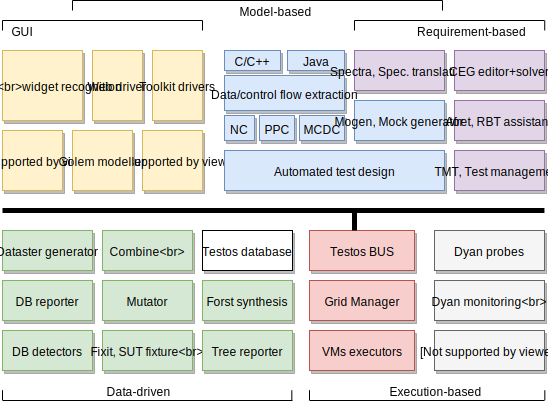
\includegraphics[width=1\textwidth]{obrazky-figures/testos.png}
	\caption{Přehled nástrojů platformy Testos}
	\label{fig_testos}
\end{figure}


\chapter{Vstupní a konfigurační soubory}
\label{chap_VstupAplikace}


\section*{Ukázka konfiguračního souboru}
\label{chap_ConfigFile}

\definecolor{maroon}{rgb}{0.5,0,0}
\definecolor{darkgreen}{rgb}{0,0.5,0}
\definecolor{darkbrown}{RGB}{139,69,19}
\definecolor{darkblue}{RGB}{25,25,112}

\lstdefinelanguage{INI}
{
  % basicstyle=\ttfamily\footnotesize,
  morecomment=[l]{;},
  morecomment=[s][\color{darkblue}\bfseries]{[}{]},
  moredelim=[s][\color{darkbrown}]{=}{\ },
  commentstyle=\color{darkgreen},
  keywordstyle={\color{maroon}\bfseries},
  morekeywords={param,parameter,parameter2},
  numbers=left,
  xleftmargin=2em,
}

\begin{lstlisting}[language={INI}, frame=single]
[ENDPOINT]
url_enum_start = <
url_enum_end = >
url_enum_separator = ,
url_variable_start = <:
url_varaible_end = :>
[METHOD]
method_enum_start = <
method_enum_end = >
method_enum_separator = ,
method_variable_start = <:
method_variable_end = :>
[HEADER]
header_enum_start = <
header_enum_end = >
header_enum_separator = ,
header_variable_start = <:
header_variable_end = :>
[BODY]
body_enum_start = <
body_enum_end = >
body_enum_separator = ,
inside_body_separator = ;
body_variable_start = <:
body_variable_end = :>
[GENERAL]
default_framework = Pytest
default_input_file = ../input/input_file.json
default_output_folder = ./result/
[COMBINATION_LIMIT]
final_tc_limit = 150
\end{lstlisting}


\section*{Ukázka vstupního soubor}

\definecolor{delim}{RGB}{20,105,176}
\definecolor{numb}{RGB}{106, 109, 32}
\definecolor{string}{rgb}{0.64,0.08,0.08}


% \lstdefinelanguage{INI}
% {
%   % basicstyle=\ttfamily\footnotesize,
%   morecomment=[l]{;},
%   morecomment=[s][\color{darkblue}\bfseries]{[}{]},
%   moredelim=[s][\color{darkbrown}]{=}{\ },
%   commentstyle=\color{darkgreen},
%   keywordstyle={\color{maroon}\bfseries},
%   morekeywords={param,parameter,parameter2},
%   numbers=left,
%   xleftmargin=2em,
% }

\lstdefinelanguage{json}{
    numbers=left,
    xleftmargin=2em,
    frame=single,
    rulecolor=\color{black},
    showspaces=false,
    showtabs=false,
    breaklines=true,
    postbreak=\raisebox{0ex}[0ex][0ex]{\ensuremath{\color{gray}\hookrightarrow\space}},
    breakatwhitespace=true,
    upquote=true,
    morestring=[b]",
    stringstyle=\color{string},
    literate=
     *{0}{{{\color{numb}0}}}{1}
      {1}{{{\color{numb}1}}}{1}
      {2}{{{\color{numb}2}}}{1}
      {3}{{{\color{numb}3}}}{1}
      {4}{{{\color{numb}4}}}{1}
      {5}{{{\color{numb}5}}}{1}
      {6}{{{\color{numb}6}}}{1}
      {7}{{{\color{numb}7}}}{1}
      {8}{{{\color{numb}8}}}{1}
      {9}{{{\color{numb}9}}}{1}
      {\{}{{{\color{delim}{\{}}}}{1}
      {\}}{{{\color{delim}{\}}}}}{1}
      {[}{{{\color{delim}{[}}}}{1}
      {]}{{{\color{delim}{]}}}}{1},
}

\begin{lstlisting}[language={json}]
{
	"test_sequence": [
		{
			"endpoint": {
		    	"values": "http://127.0.0.1:5000/api/v1/calculator",
			    "local_params": []
		    },
		    "method": {
				"values": "<:method:>",
				"local_params": []
			},
			"header": {
				"values": "<>",
				"local_params": [
					{
						"values": ["header.yaml"]
					}
				]
			},
			"body": {
				"values": "",
				"local_params": []
			},
			"t-way": 2
		}
	],
	"t-way": 2,
	"global_params": {
		"method": ["GET","POST"]
	}
}
\end{lstlisting}

% \chapter{Výstup aplikace}
% \begin{lstlisting}[language=Python, frame=single, numbers=left, xleftmargin=2em]
% from unittest import TestCase
% from json import dumps
% import requests

% class ContextClass(object):
%     def __init__(self, request, endpoint_params, method_params, header_params, body_params):
%         self.endpoint = request[0]
%         self.method = request[1]
%         self.header = request[2]
%         self.body = request[3]
%         # parameters
%         self.endpoint_params = endpoint_params
%         self.method_params = method_params
%         self.header_params = header_params
%         self.body_params = body_params

% def setup():
%     #####################################
%     # TODO: HERE IS YOUR CODE
%     # Insert your code to define prerequisities of SUT
%     None

% def verify(test_case, request_id, response, context):
%     """
%     Method to describe the expected values for all test cases
%     Take into account that these if-else statements will be duplicated for all test cases
%     You can also rewrite whole method from scretch and use [TODO:] argument while calling 
%     suiter to avoid code duplicate 
%     """
%     if test_case == "test_case_001":
%         if request_id == "call_1":
%             # Test Case Information
%             # endpoint = http://127.0.0.1:5000/api/v1/calculator?operation=add&num1=0&num2=0
%             # method = GET
%             # header = {"Content-type": "json", "testInt": "12", "dalsiTest": "test"}
%             # body = ./body_files/request_1_body_1
%             assert response.status_code == 200
%         elif request_id == "call_2":
%             # Test Case Information
%             # endpoint = http://127.0.0.1:5000/api/v1/calculator?operation=add&num1=0&num2=0
%             # method = GET
%             # header = {"Content-type": "json", "testInt": "12", "dalsiTest": "test"}
%             # body = ./body_files/request_2_body_1
%             assert response.status_code == 200
%         else:
%             raise Exception("Should have never gotten here: [{},{}]".format(test_case,request_id))

% def teardown():
%     #####################################
%     # TODO: HERE IS YOUR CODE
%     # Write a code to set the SUT to it's original state
%     # if it is dependend on given test_case, add a 'test_case' parameter to this function
%     # and write a code for all test_cases
%     ## def teardown(test_case):
%     None

% def all_test_cases(test_case, request_id):
%     """
%     List of all test cases in this test suite
%     """
%     if test_case == "test_case_001":
%         if request_id == "call_1":
%             url = "http://127.0.0.1:5000/api/v1/calculator?operation=add&num1=0&num2=0"
%             method = "GET"
%             header = {"Content-type": "json", "testInt": "12", "dalsiTest": "test"}
%             body = "./body_files/request_1_body_1"
%         elif request_id == "call_2":
%             url = "http://127.0.0.1:5000/api/v1/calculator?operation=add&num1=0&num2=0"
%             method = "GET"
%             header = {"Content-type": "json", "testInt": "12", "dalsiTest": "test"}
%             body = "./body_files/request_2_body_1"
%         else:
%             raise Exception("Should have never gotten here: [{},{}]".format(test_case,request_id))
%     else:
%         raise Exception("Should have never gotten here: [{},{}]".format(test_case,request_id))

%     return (url, method, header, body)

% class TestClass(TestCase): 
%     def test_sequence_001(self):
%         ### SUT Setup ###
%         setup()
%         ### 1. Request ###
%         call = all_test_cases("test_case_001", "call_1")
%         with open(call[3],'rb') as payload:
%             response = requests.request(call[1], call[0], headers=call[2], data=payload)
%         verify("test_case_001", "call_1", response, call)
%         ### 2. Request ###
%         call = all_test_cases("test_case_001", "call_2")
%         with open(call[3],'rb') as payload:
%             response = requests.request(call[1], call[0], headers=call[2], data=payload)
%         verify("test_case_001", "call_2", response, call)
%         ### SUT Teardown ###
%         teardown()
% \end{lstlisting}





\chapter{Šablona testovacího skriptu pro Python}
\label{cahp_sablona}

\definecolor{maroon}{rgb}{0.5,0,0}
\definecolor{darkgreen}{rgb}{0,0.5,0}
\definecolor{darkbrown}{RGB}{139,69,19}
\definecolor{darkblue}{RGB}{25,25,112}

\begin{lstlisting}[language=Python, basicstyle=\ttfamily\scriptsize,numbers=left,xleftmargin=2em,frame=single]
from unittest import TestCase
from json import dumps
import requests

class ContextClass(object):
    def __init__(self, request, endpoint_params, method_params, header_params, body_params):
        self.endpoint = request[0]
        self.method = request[1]
        self.header = request[2]
        self.body = request[3]
        # parameters
        self.endpoint_params = endpoint_params
        self.method_params = method_params
        self.header_params = header_params
        self.body_params = body_params

def setup():
    #####################################
    # TODO: HERE IS YOUR CODE
    # Insert your code to define prerequisities of SUT
    None

def verify(test_case, request_id, response, context):
    """ Method to describe the expected values for all test cases """
<VERIFY>    
    
def teardown():
    #####################################
    # TODO: HERE IS YOUR CODE
    # Write a code to set the SUT to it's original state
    None

def all_test_cases(test_case, request_id):
    """ List of all test cases in this test suite """
<TEST_CASE_LIST>
    return (url, method, header, body)

class TestClass(TestCase): 
<TEST_SEQUENCE>
\end{lstlisting}


\chapter{Obsah těla HTTP požadavku odeslaného nástroji Combine}
\label{combine_body}

\definecolor{delim}{RGB}{20,105,176}
\definecolor{numb}{RGB}{106, 109, 32}
\definecolor{string}{rgb}{0.64,0.08,0.08}

\lstdefinelanguage{json}{
    numbers=left,
    xleftmargin=2em,
    frame=single,
    rulecolor=\color{black},
    showspaces=false,
    showtabs=false,
    breaklines=true,
    postbreak=\raisebox{0ex}[0ex][0ex]{\ensuremath{\color{gray}\hookrightarrow\space}},
    breakatwhitespace=true,
    upquote=true,
    morestring=[b]",
    stringstyle=\color{string},
    literate=
     *{0}{{{\color{numb}0}}}{1}
      {1}{{{\color{numb}1}}}{1}
      {2}{{{\color{numb}2}}}{1}
      {3}{{{\color{numb}3}}}{1}
      {4}{{{\color{numb}4}}}{1}
      {5}{{{\color{numb}5}}}{1}
      {6}{{{\color{numb}6}}}{1}
      {7}{{{\color{numb}7}}}{1}
      {8}{{{\color{numb}8}}}{1}
      {9}{{{\color{numb}9}}}{1}
      {\{}{{{\color{delim}{\{}}}}{1}
      {\}}{{{\color{delim}{\}}}}}{1}
      {[}{{{\color{delim}{[}}}}{1}
      {]}{{{\color{delim}{]}}}}{1},
}

\begin{lstlisting}[language={json}]
{
    "name": "SUT name",
    "t_strength": "2",
    "dont_care_values": "no",
    "values": "values",
    "parameters": [
        {
            "identificator": "ArrayType",
            "type": "enum",
            "blocks": [
                "[1,2,3]",
                "[a,b,c]",
                "[A,B,C]"
            ]
        },
        {
            "identificator": "IntegerType",
            "type": "enum",
            "blocks": [
                "1",
                "2"
            ]
        }
    ],
    "constraints": []
}
\end{lstlisting}